\documentclass{exam}
\usepackage[utf8]{inputenc}
\usepackage{lmodern}
\usepackage{microtype}

% \usepackage[parfill]{parskip}
\usepackage[dvipsnames]{xcolor}
\usepackage{amsmath}
\usepackage{amsfonts}
\usepackage{amsthm}
\usepackage{siunitx}
\DeclareSIUnit\year{yr}
\DeclareSIUnit\foot{ft}
\DeclareSIUnit\litre{\liter}

\usepackage{skull}

\usepackage{pgfplots}
\usepgfplotslibrary{polar}
\pgfplotsset{compat=1.11}
\usepackage{graphicx}
\usepackage{sidecap}
\sidecaptionvpos{figure}{c}
\usepackage{float}
\usepackage{gensymb}
\usepackage{tkz-euclide}
\usetkzobj{all}
\usepackage{commath}
\usepackage{hyperref}
\usepackage{enumitem}
\usepackage{wasysym}
\usepackage{multicol}
\usepackage{mathtools}
\usepackage{tcolorbox}
\usepackage{tabularx}
\usepackage[version=4]{mhchem}
\usepackage{changepage}
\usepackage{listings}
\lstset{basicstyle=\ttfamily\linespread{0.8}\small}

\renewcommand*{\thefootnote}{\fnsymbol{footnote}}

\newtheorem*{thm}{Theorem}
\newtheorem*{iden}{Identity}
\newtheorem*{lemma}{Lemma}
\newtheorem{obs}{Observation}
\theoremstyle{definition}
\newtheorem*{defn}{Definition}
\newtheorem*{ex}{Example}
\newtheorem{con}{Construction}
\newtheorem*{alg}{Algorithm}

\newtheoremstyle{break}
  {\topsep}{\topsep}%
  {\itshape}{}%
  {\bfseries}{}%
  {\newline}{}%
\theoremstyle{break}
\newtheorem*{bthm}{Theorem}

% russian integral
\usepackage{scalerel}
\DeclareMathOperator*{\rint}{\scalerel*{\rotatebox{17}{$\!\int\!$}}{\int}}

% \DeclareMathOperator*{\rint}{\int}

\pgfplotsset{vasymptote/.style={
    before end axis/.append code={
        \draw[densely dashed] ({rel axis cs:0,0} -| {axis cs:#1,0})
        -- ({rel axis cs:0,1} -| {axis cs:#1,0});
    }
}}

% \pointsinrightmargin
\boxedpoints
\pointname{}

\newcommand{\questioA}{\question[\texttt{\textbf{\color{Cerulean} A}}]}
\newcommand{\questioM}{\question[\texttt{\textbf{\color{PineGreen} M}}]}
\newcommand{\questioE}{\question[\texttt{\textbf{\color{WildStrawberry} E}}]}
\newcommand{\questioS}{\question[\texttt{\textbf{\color{Goldenrod} S}}]}
\newcommand{\questioO}{\question[\texttt{\textbf{\color{BurntOrange} O}}]}

\newcommand{\parA}{\part[\texttt{\textbf{\color{Cerulean} A}}]}
\newcommand{\parM}{\part[\texttt{\textbf{\color{PineGreen} M}}]}
\newcommand{\parE}{\part[\texttt{\textbf{\color{WildStrawberry} E}}]}
\newcommand{\parS}{\part[\texttt{\textbf{\color{Goldenrod} S}}]}
\newcommand{\parO}{\part[\texttt{\textbf{\color{BurntOrange} O}}]}

\newcommand{\subparA}{\subpart[\texttt{\textbf{\color{Cerulean} A}}]}
\newcommand{\subparM}{\subpart[\texttt{\textbf{\color{PineGreen} M}}]}
\newcommand{\subparE}{\subpart[\texttt{\textbf{\color{WildStrawberry} E}}]}
\newcommand{\subparS}{\subpart[\texttt{\textbf{\color{Goldenrod} S}}]}
\newcommand{\subparO}{\subpart[\texttt{\textbf{\color{BurntOrange} O}}]}

\newcommand{\mainHeader}[2]{\section*{NCEA Level 2 Mathematics\\#1. #2}}
\newcommand{\mainHeaderHw}[2]{\section*{NCEA Level 2 Mathematics (Homework)\\#1. #2}}


\begin{document}

\mainHeaderHw{10}{Negative and Fractional Powers}
\subsection*{Reading}
\emph{Editorial note: rather than boring you with more `applications of exponents' (I listed most of the interesting
ones last week), here's a little history.}

In the May 1690 issue of the \textit{Acta Eroditorum}, Jakob Bernoulli, the discoverer of $ e $, revisited a question that had
been puzzling mathematicians for a century. What is the correct geometry of the shape made by a piece of string when it is hanging
between two points? This curve --- called the `catenary', from the Latin \textit{catena}, chain --- is produced when material is
suspended by its own weight.

The curve whose identity Jakob Bernoulli so ardently sought turned out to have a hidden ingredient, $ e $, the number he had
uncovered in a different context [compound interest].

In modern notation, the equation for the catenary is
\begin{displaymath}
  y = \frac{e^{ax} + e^{-ax}}{2a},
\end{displaymath}
where $ a $ is a constant that changes the scale of the curve. The bigger $ a $ is, the further apart the two ends of the hanging
string are.

Look closely at the equation. The term $ e^{ax} $ represents pure exponential growth, and the term $ e^{-ax} $ pure exponential
decay. The equation adds them together, and then divides by two, which is a familiar arithmetical operation: adding two values
and then halving the result is what we do when we want to find their average. In other words, the catenary is the average
of the curves of exponential growth and decay, as illustrated below. Every point on the U falls exactly halfway between the
two exponential curves.

Whenever we see a circle, we see $ \pi $, the ratio of the circumference to the diameter. And whenever we see a hanging chain,
a dangling spider's thread or the dip of an empty washing line, we see $ e $.

\begin{center}
\fbox{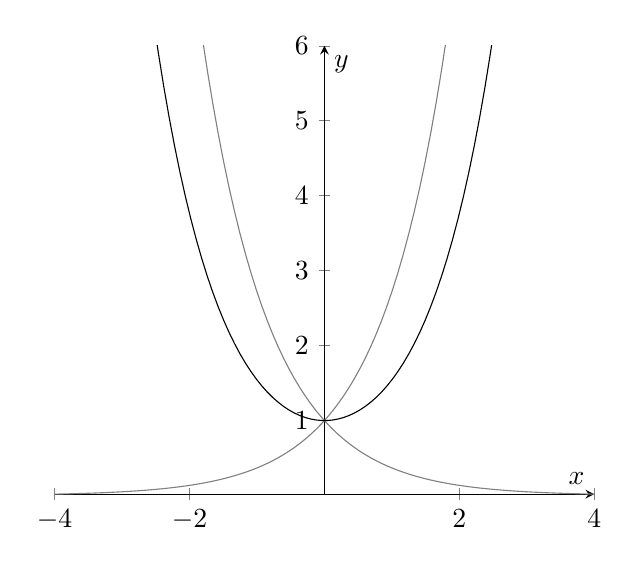
\begin{tikzpicture}
  \begin{axis}[
    /pgf/number format/1000 sep={},
    axis lines = center,
    ymax = 6,
    xlabel = $ x $,
    ylabel = $ y $
  ]
    \addplot[domain = -4:4, color = gray, samples = 100] {exp(x)};
    \addplot[domain = -4:4, color = gray, samples = 100] {exp(-x)};
    \addplot[domain = -4:4, color = black, samples = 100] {(exp(x) + exp(-x))/2};
  \end{axis}
\end{tikzpicture}}
\end{center}

\begin{flushright}
  Adapted from \textit{Alex Through the Looking-Glass}, by Alex Bellos (pp.150-2).
\end{flushright}

\clearpage
\subsection*{Questions}
\begin{questions}
  \question Expand and simplify, writing with only positive exponents.
    \begin{parts}
      \part $ \dfrac{(3 + x^{3/2})(3 - x^{3/2})}{x^{-4}} $
      \part $ \dfrac{x(y^3 + \sqrt{y}) + y^3}{y} - xy^{-(1/2)} $
    \end{parts}
  \question Find all solutions to $ 8x^{3} + 64 = 16\sqrt{8}x^{3/2} $.
  \question Challenge question: we have seen that $ \sqrt{2} $ is irrational; that is, $ 2^{1/2} $ is irrational
            and so it is possible for $ a^b $ to be irrational when both $ a $ and $ b $ are
            rational. Is it possible for $ a^b $ to be \emph{rational} when both $ a $ and $ b $
            are \emph{irrational}?
\end{questions}

\end{document}
